A farmer has a set of fields, each of which is surrounded by cypress trees. Also, the farmer has a set of strips of land, each of which has a row of cypress trees. In both fields and strips, between every two consecutive cypress trees is a single olive tree. All of the farmer's cypress trees either surround a field or are in a strip and all of the farmer's olive trees are between two consecutive cypress trees in a field or in a strip. 

One day the farmer became very ill and he felt that he was going to die. A few days before he passed away he called his eldest son and told him, "I give you any $Q$ cypress trees of your choice and all the olive trees which are between any two consecutive cypress trees you have chosen." 

From each field and from each strip the son can pick any combination of cypress trees. Since the eldest son loves olives he wants to pick the Q cypress trees which will allow him to inherit as many olive trees as possible. 

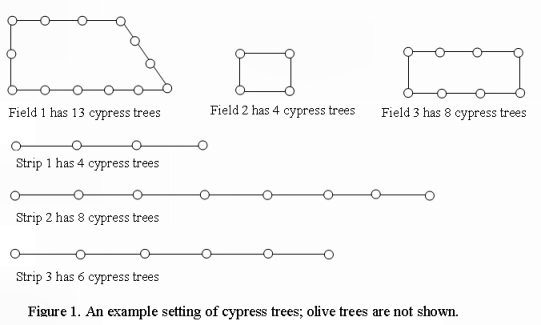
\includegraphics{cypress.jpg}

In Figure 1, assume that the son is given $Q=17$ cypress trees. To maximize his olive inheritance he should choose all the cypress trees in Field 1 and Field 2, inheriting 17 olive trees. 

You are to write a program which, given the information about the fields and the strips and the number of cypress trees the son can pick, determines the largest possible number of olive trees the son may inherit.  